\section{Versuchsziele}
\begin{figure}[!h]
		\centering
		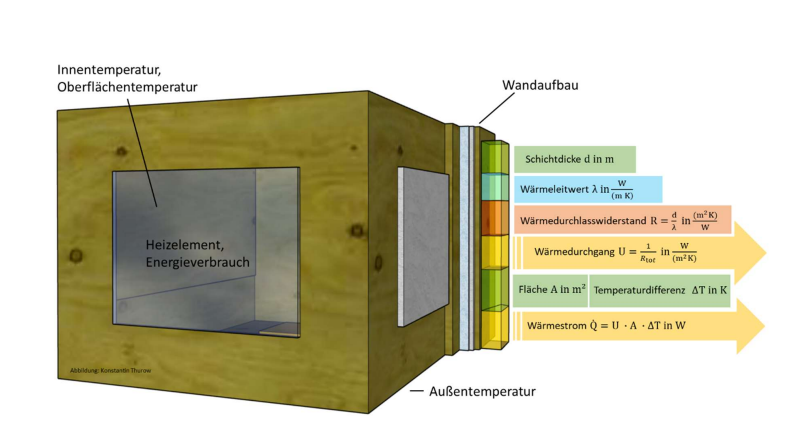
\includegraphics[width=0.7\textwidth]{Abbildungen/Thurow_Deckblatt}
		\caption{Animation des Versuchsaufbaus [Versuchsanleitung] }
		\label{fig:Versuchsaufbau}
\end{figure}

Mit Blick auf die Ziele der Bundesregierung den Endenergieverbrauch bis 2030 um 24\% zu senken gewinnt Energieeffizienz im Bausektor mit rasender Geschwindigkeit an Relevanz. Die Effizienzklassen für Neubauten legen den Fokus auf Dämmungen und können so in den nächsten Jahrzehnten viel Gas und Kohle einsparen. Dieser Versuch soll ein Verständnis für Dämmstoffe und die Klassifikation dieser durch den Wärmedurchgangskoeffizienten (U-Wert) schaffen.  Der Versuchsaufbau besteht aus einem Modellhaus (\autoref{fig:Versuchsaufbau}) mit austauschbaren Wänden, einem abnehmbaren Dach und einer Glühlampe als Wärmequelle. Ziel ist es, aus den aufgenommenen Temperaturdifferenzen, in der Auswertung die Wärmeleitfähigkeit und den Wärmedurchgang der einzelnen Materialien zu bestimmen.\\\\
Aus Erfahrungswerten und bisherigen Vorlesungsveranstaltungen lässt sich vermuten, dass einige der Materialien Wärme besser leiten als andere. Während Polysterol, oftmals auch als Dämmstoff genutzt, eine schlechte Wärmeleitfähigkeit aufweisen wird, leitet das Floatglas Wärme wahrscheinlich am besten und hat so auch den größten U-wert. Erwartbar ist außerdem, dass die U-werte in der zweiten Messung geringer sein werden als in der ersten da das Schichtholz durch eine Dämmung ergänzt wurde.